\chapter{\label{background}Background}

\section{Fermionic Simulation Scheme}

\begin{enumerate}
    \item Map some fermionic state, usually in the occupation number representation to a qubit state.
    \item This mapping must be done in such a way as to preserve the fermionic anti-commutation relations, and hence preserve Pauli antisymmetry.
    \item Common fermionic-qubit mappings include Jordan-Wigner and Bravyi-Kitaev.
    \item We then act on the qubit state with a unitary operator that represents a fermionic operator.
    \item The resulting qubit state is then decoded to yield the resultant fermionic state.
    \item A successful simulation scheme is one that reproduces the action of the fermionic operator
\end{enumerate}

\section{Occupation Number Representation}
In second quantisation, wavefunctions are represented in the occupation number representation.
\begin{equation*}
    \ket\psi = \ket{f_{n-1} \dots f_{0}} \qquad \text{where } f_{j} \in {0, 1}
\end{equation*}

Where $\ket\psi$ represents a Slater determinant usually constructed from Hartree-Fock spin orbitals.

This means that given $n$ spin-orbitals, there exist $2^n$ electronic basis states.
\begin{equation*}
    \ket\psi = \ket{0 \dots 10} =
    \begin{pmatrix} 0 \\ 1 \\ \vdots \\ \vdots \\ \vdots \\ 0 \end{pmatrix} \qquad
\end{equation*}

Fermionic interactions can be represented in terms of the creation and annhilation operators $a_j^\dagger$ and $a_j$. \bigskip

Consider the excitation of an electron in the lowest spin-orbital to the second spin-orbital.

\begin{equation*}
\begin{gathered}
    \ket{\psi_1} \rightarrow \ket{\psi_2} \\
    a_2^\dagger \, a_1 \ket{001} = \ket{010}
\end{gathered}
\end{equation*}

Importantly, due to the exchange anti-symmetry of fermions, the action of the creation/annhilation operators introduces a phase to the electronic wavefunction.

\begin{align*}
    a_j^\dagger \ket{f_{n-1} \dots
    f_{j+1},\,\, 0,\,\, f_{j-1} \dots f_0} &=
    (-1)^{\sum_{s=0}^{j-1} f_s}
    \ket{f_{n-1} \dots f_{j+1},\,\, 1,\,\, f_{j-1} \dots f_0} \\
    %
    a_j^\dagger \ket{f_{n-1} \dots f_{j+1},\,\, 1,\,\, f_{j-1}
    \dots f_0} &= \vec 0 \\
    %
    a_j \ket{f_{n-1} \dots f_{j+1},\,\, 1,\,\, f_{j-1} \dots f_0} &=
    (-1)^{\sum_{s=0}^{j-1} f_s}
    \ket{f_{n-1} \dots f_{j+1},\,\, 0,\,\, f_{j-1} \dots f_0} \\
    %
    a_j \ket{f_{n-1} \dots f_{j+1},\,\, 0,\,\, f_{j-1} \dots f_0} &= \vec 0
\end{align*}

The phase introduced depends on the \textbf{parity} of the spin-orbitals preceding spin-orbital $j$.

In the second-quantisation, this anti-symmetry is expressed in terms of the anti-commutation of creation and annhilation operators.
\begin{align*}
    \{ \hat a_{j}, \hat a_{k} \} &=
    \hat a_{j} \hat a_{k} + \hat a_{k} \hat a_{j} = 0 \\
    %
    \{ \hat a_{j}^{\dagger}, \hat a_{k}^{\dagger} \} &=
    \hat a_{j}^\dagger \hat a_{k}^\dagger + \hat a_{k}^\dagger \hat a_{j}^\dagger = 0 \\
    %
    \{ \hat a_{j}, \hat a_{k}^{\dagger} \} &= \hat a_{j} \hat a_{k}^\dagger + \hat a_{k}^\dagger \hat a_{j} = \delta_{jk} \hat{1}
\end{align*}

In fact, we find that the phase factor discussed in the previous section is automatically kept track of by these relations.

The Hamiltonian in second quantisation can also be expressed in terms of the creation and annhilation operators.

\begin{equation*}
    \hat H =
    \sum_{ij} h_{ij} a^\dagger_i a_j +
    \frac{1}{2} \sum_{ijkl} h_{ijkl} a^\dagger_i a^\dagger_j a_k a_l +
    h_\text{Nu}
\end{equation*}

Where $h_{ij}$ (one-electron overlap integral) and $h_{ijjk}$ (two-electron overlap integral) are computed classically.


\section{Fermion-Qubit Encodings}
The form of the occupation number representation basis suggests the following identification between electronic states and qubit states.

\begin{equation*}
    \ket{f_{n-1} \dots f_{0}} \quad\rightarrow\quad \ket{q_{n-1} \dots q_{0}}
\end{equation*}

That is, we allow each qubit to store the occupation number of a given spin-orbital.

% In order to actually simulate a Hamiltonian...

We must map the fermionic creation and annhilation operators onto qubit operators.
\begin{equation*}
    \hat a^\dagger \rightarrow \hat Q^+ \qquad
    \hat a \rightarrow \hat Q
\end{equation*}

And these operators must behave in the same way as their fermionic analogues.

\begin{equation*}
\begin{gathered}
    \hat Q^+ \ket 0 = \ket 1 \qquad \hat Q^+ \ket 1 = 0 \\
    \hat Q \ket 1 = \ket 0 \qquad \hat Q \ket 0 = 0
\end{gathered}
\end{equation*}

Note that we must also preserve the fermionic anti-commutation relations in the qubit operators.

\begin{equation*}
\begin{gathered}
    \{ \hat Q_{j}, \hat Q_{k} \} = 0 \qquad
    %
    \{ \hat Q_{j}^{\dagger}, \hat Q_{k}^{\dagger} \} = 0 \\
    %
    \{ \hat Q_{j}, \hat Q_{k}^{\dagger} \} = \delta_{jk}
\end{gathered}
\end{equation*}\medskip

This ensures the fermionic exchange anti-symmetry of our qubit state vector.

We can do this using the \textbf{Jordan-Wigner} transformation by expressing the fermionic operators as a linear combination of the Pauli matrices.
\begin{figure}
    \begin{equation*}
    \begin{gathered}
        \hat Q^+ = \ket 1 \bra 0 = \frac{1}{2} (X - iY) \\
        \hat Q = \ket 0 \bra 1 = \frac{1}{2} (X + iY) 
    \end{gathered}
    \end{equation*}
    \caption{Single qubit creation and annhilation operators.}
\end{figure}

We can see that these do indeed behave in the same way as their fermionic analogues,

\begin{equation*}
\begin{gathered}
    \hat Q^+ \ket 0 = (\ket 1 \bra{0})\ket{0} = \ket 1 \qquad
    \hat Q^+ \ket 1 = (\ket 1 \bra{0})\ket{1} = 0 \\
    %
    \hat Q \ket 1 = (\ket 0 \bra{1})\ket{1} = \ket 0 \qquad
    \hat Q \ket 0 = (\ket 0 \bra{1})\ket{0} = 0
\end{gathered}
\end{equation*}

When dealing with \textbf{multiple-qubits}, we must also account for the occupation parity of the qubits preceding the target qubit $j$.

\begin{equation*}
    a_j^\dagger \ket{f_{n-1} \dots f_{j+1},\,\, 0,\,\, f_{j-1} \dots f_0} =
    (-1)^{\sum_{s=0}^{j-1} f_s}
    \ket{f_{n-1} \dots f_{j+1},\,\, 1,\,\, f_{j-1} \dots f_0}
\end{equation*}

We do this by introducing a string of Pauli Z operators that computes the parity of the qubits preceding the target qubit.

\begin{equation*}
\begin{gathered}
    \hat a_j^+ = \frac{1}{2} (X - iY) \prod_{k=1}^{j-1} Z_k \qquad
    \hat a_j = \frac{1}{2} (X + iY) \prod_{k=1}^{j-1} Z_k \\
    \text{Where $\prod$ is the tensor product.}
\end{gathered}
\end{equation*}

A more compact notation is,

\begin{equation*}
    \hat a_j^+ = \frac{1}{2} (X - iY) \otimes Z^\rightarrow_{j-1} \qquad
    \hat a_j = \frac{1}{2} (X + iY) \otimes Z^\rightarrow_{j-1}
\end{equation*}\medskip

Where $Z^\rightarrow_{i}$ is the parity operator with eigenvalues $\pm 1$, and ensures the correct phase is added to the qubit state vector.
\begin{equation*}
    Z^\rightarrow_{i} = Z_i \otimes Z_{i-1} \otimes \dots \otimes Z_0
\end{equation*}

For instance, the creation operator $a^\dagger_3$ maps to the following Pauli string,

\begin{align*}
    \hat a_3^\dagger &=
    \frac{1}{2} (X_3 - iY_3) \otimes Z_2 \otimes Z_1 \otimes Z_0 \\
    %
    \hat a_3^\dagger &=
    \frac{1}{2} ( X_3 \otimes Z_2 \otimes Z_1 \otimes Z_0 ) -
    \frac{1}{2} i ( Y_3 \otimes Z_2 \otimes Z_1 \otimes Z_0 )
\end{align*}

Usually we drop the subscript specifying the orbital acted on.

\section{Unitary Coupled Cluster}

Within the traditional coupled-cluster framework, the ground electronic state is prepared by applying the CC operator to a reference state (usually Hartree-Fock).

\begin{equation*}
    \ket\psi = e^{\hat T} \ket{\phi_0}
\end{equation*}

Where $\hat T$ is the cluster excitation operator.

Quantum gates, however, must be unitary operators, so instead, we work within the UCC framework.

\begin{equation*}
    \ket\psi = e^{\hat T} \ket{\phi_0}
\end{equation*}

Where $\hat T$ is now an \textbf{anti-Hermitian} operator, and $e^{\hat T}$ is unitary.

In general, we can prepare exact electronic states by applying a sequence of $k$ parametrised unitary operators to our reference state.

\begin{equation*}
\begin{gathered}
    \ket\psi = \prod_i^k U_i(\theta_i) \ket{\phi_0} \\
    \text{Where $U_i(\theta_i)$ is a parametrised unitary operator}
\end{gathered}
\end{equation*}\smallskip

The parameters $\theta_i$ are then optimised to find the ground state energy.

General fermionic single and double excitation operators are defined as,
\begin{equation*}
    a_q^\dagger a_p \text{ and } a_r^\dagger a_s^\dagger a_q a_p
\end{equation*}

Exciting one electron from $p$ to $q$, and two electrons from $p, q$ to $r, s$ respectively.

Taking a linear combination of these, we obtain \textbf{anti-Hermitian} fermionic single and double excitation operators.
\begin{equation*}
\begin{gathered}
    \hat\kappa_p^q = a_q^\dagger a_p - a_p^\dagger a_q \\
    %
    \hat\kappa_{pq}^{rs} =
    a_r^\dagger a_s^\dagger a_q a_p - a_p^\dagger a_q^\dagger a_s a_r
\end{gathered}
\end{equation*}\smallskip

Such that upon exponentiating, we obtain \textbf{unitary} operators.

\begin{equation*}
    U^q_p = e^{\hat\kappa_p^q} \qquad
    %
    U_{pq}^{rs} = e^{\hat\kappa_{pq}^{rs}}
\end{equation*}

Recalling the Jordan-Wigner encoding for the creation and annhilation operators,

\begin{equation*}
    \hat a_j^+ = \frac{1}{2} (X - iY) \otimes Z^\rightarrow_{j-1} \qquad
    \hat a_j = \frac{1}{2} (X + iY) \otimes Z^\rightarrow_{j-1}
\end{equation*}

The anti-Hermitian fermionic single and double excitation operators $\kappa_p^q$ and $\kappa_{pq}^{rs}$
\begin{align*}
    F_p^q = \frac{i}{2} & (Y_p X_q - X_p Y_q) \prod_{k=p+1}^{q-1} Z_k \\
    %
    F_{pq}^{rs} = \frac{i}{8} (
      & X_p X_q Y_s X_r +
        Y_p X_q Y_s Y_r +
        X_p Y_q Y_s Y_r +
        X_p X_q X_s Y_r - \\
      & Y_p X_q X_s X_r -
        X_p Y_q X_s X_r -
        Y_p Y_q Y_s X_r -
        Y_p Y_q X_s Y_r )
    \prod_{k=p+1}^{q-1} Z_k
    \prod_{l=r+1}^{s-1} Z_l
\end{align*}

Multiplying by $\theta$ and exponentiating yields the parametrised unitary qubit operators,

\begin{equation*}
    U^q_p (\theta) =
    \text{exp} \left( i
    \frac{\theta}{2} (Y_p X_q - X_p Y_q) \prod_{k=p+1}^{q-1} Z_k \right)
\end{equation*}

\begin{equation*}
    U^{rs}_{pq} (\theta) = \text{exp} \left( i \frac{\theta}{8} (
    X_p X_q Y_s X_r
    + \dots -
    Y_p Y_q Y_s X_r -
    Y_p Y_q X_s Y_r )
    \prod_{k=p+1}^{q-1} Z_k
    \prod_{l=r+1}^{s-1} Z_l
    \right)
\end{equation*}

To summarise, we constructed anti-Hermitian single and double excitation operators from a linear combination of fermionic excitation operators,

\begin{equation*}
    \hat\kappa_p^q = a_q^\dagger a_p - a_p^\dagger a_q \qquad
    %
    \hat\kappa_{pq}^{rs} =
    a_r^\dagger a_s^\dagger a_q a_p - a_p^\dagger a_q^\dagger a_s a_r
\end{equation*}\smallskip

We then mapped these to qubit operators using the Jordan-Wigner transformation,
\begin{equation*}
    \hat\kappa_p^q \xrightarrow{\text{JW}} F_p^q \qquad\qquad
    \hat\kappa_{pq}^{rs} \xrightarrow{\text{JW}} F_{pq}^{rs}
\end{equation*}

And finally, we exponentiated to yield the parametrised unitary qubit operators.
\begin{equation*}
    U^q_p (\theta) = e^{\theta^q_p F_p^q} \qquad
    %
    U^{rs}_{pq}(\theta) = e^{\theta_{pq}^{rs} F_{pq}^{rs}}
\end{equation*}

\section{DISCO-VQE}

\subsubsection{Excitation Operators in ZXC}

Let's look again at the parametrised single-body unitary operator,

\begin{equation*}
\begin{gathered}
    U^q_p (\theta) =
    \text{exp} \left( i
    \frac{\theta}{2} (Y_p X_q - X_p Y_q) \prod_{k=p+1}^{q-1} Z_k \right) \\
    %
    U^q_p (\theta) =
    \left( \text{exp} \left[
    i \frac{\theta}{2} Y_p X_q \prod_{k=p+1}^{q-1} Z_k \right] \right)
    %
    \left( \text{exp} \left[ -
    i \frac{\theta}{2} X_p Y_q \prod_{k=p+1}^{q-1} Z_k \right] \right)
\end{gathered}
\end{equation*}

The first exponential term can be implemented by the following phase gadget.
\begin{equation*}
    \text{exp} \left( i
    \frac{\theta}{2} Y_p X_q \prod_{k=p+1}^{q-1} Z_k \right)
\end{equation*}

% \begin{figure}
% \centering
%     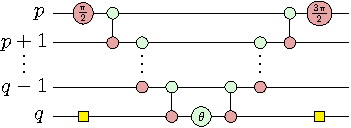
\includegraphics[width=8cm]{figures/zxc/yx_cnot}
% \end{figure}

% Rotation of qubit $p$ into $Y$ basis and rotation of qubit $q$ into $X$ basis, followed rotations back into $Z$ basis at the end of the circuit.

% Left CNOT ladder construction calculates the parity of the qubit state, and applies a rotation in the $Z$ basis if the parity is odd.

% Right CNOT ladder construction to uncompute.

Whilst the second exponential term can be implemented by the phase gadget.
\begin{equation*}
    \text{exp} \left( - i
    \frac{\theta}{2} X_p Y_q \prod_{k=p+1}^{q-1} Z_k \right)
\end{equation*}

% \begin{figure}
% \centering
%     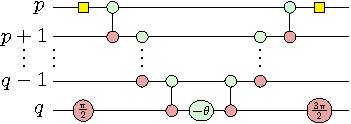
\includegraphics[width=8cm]{figures/zxc/xy_cnot}
% \end{figure}

%%% ----- %%%

Together, they constitute the single-body unitary excitation operator $U^q_p (\theta)$

% \begin{figure}
% \centering
%     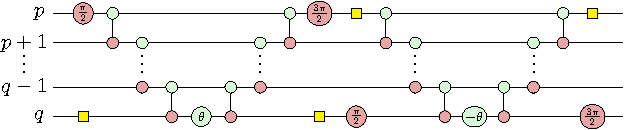
\includegraphics[width=14cm]{figures/zxc/full_cnot}
% \end{figure}

By defining the ordering of spin-orbitals such that adjacent spin-orbitals share the same spatial orbital, adjacent single-body operators commute.

\begin{equation*}
    \left[ \hat\kappa_p^q, \hat\kappa_{p+1}^{q+1} \right] = 0
\end{equation*}\smallskip

The same is therefore true for the resulting qubit operators,

\begin{equation*}
\begin{gathered}
    \left[ F_p^q, F_{p+1}^{q+1} \right] = 0 \\
    p, q \in \text{even} \qquad p+1, q+1 \in \text{odd}
\end{gathered}
\end{equation*}

This allows us to define the parametrised unitary qubit operators in terms of spin-adapted excitation operators.

\begin{equation*}
    U^q_p (\theta) = \text{exp}
    \left[ \theta \left( F_p^q + F_{p+1}^{q+1} \right) \right]
\end{equation*}

In other words, since $F_p^q$ and $F_{p+1}^{q+1}$ commute, we can think of them as a single operator with a single parameter.

%%% ----- %%%

Spin-adapted single-body unitaries are implemented with \textbf{four} phase gadgets. \bigskip

% \begin{figure}
% \centering
%     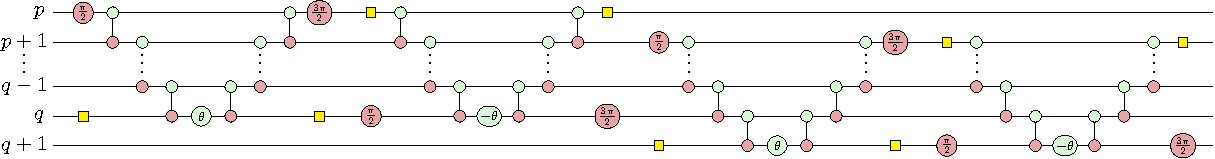
\includegraphics[width=14cm]{figures/zxc/full_spin_adapted}
%     \caption{Circuit implementation of a spin-adapted single-body unitary.}
% \end{figure}

It turns out that in the ZX calculus, phase gadgets can be rewritten in the following way. \smallskip

% \begin{figure}
% \centering
%     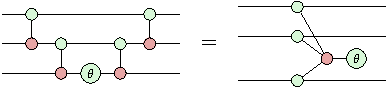
\includegraphics[width=9cm]{figures/zxc/phase_gadget}
% \end{figure}

For two qubits, we can prove this correspondence easily.

% \begin{figure}
% \centering
%     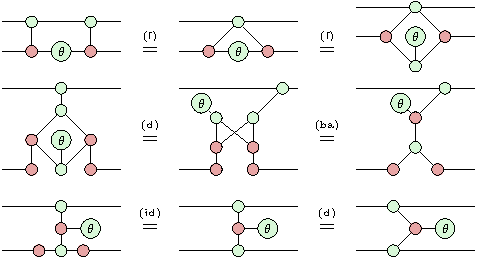
\includegraphics[width=9cm]{figures/zxc/phase_gadget_proof}
% \end{figure}

For three or more qubits... (proof by induction) \smallskip

% \begin{figure}
% \centering
%     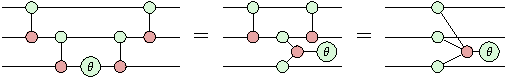
\includegraphics[width=13cm]{figures/zxc/phase_gadget_proof2}
% \end{figure}

So our spin-adapted single-body unitary implemented by the following circuit...

% \begin{figure}
% \centering
%     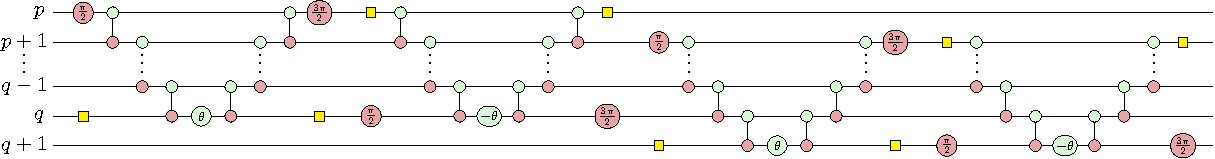
\includegraphics[width=14cm]{figures/zxc/full_spin_adapted}
% \end{figure}

...can be rewritten as the following ZX diagram.

% \begin{figure}
% \centering
%     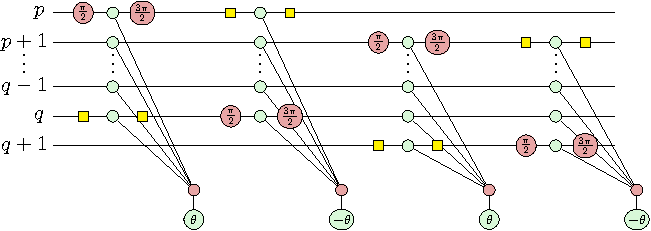
\includegraphics[width=11cm]{figures/zxc/full_spin_adapted_zx}
% \end{figure}

% \section{Quantum Computation}
% \subsection{Fundamentals}
% \subsubsection{Basis States}
% \subsubsection{Single-Qubit Statevector}
% \subsubsection{Multi-Qubit Statevector}

% \subsection{Quantum Gates}
% \subsubsection{Pauli Gates}
% \subsubsection{Rotation Gates}
% \subsubsection{Clifford Gates}

\section{ZX Calculus}
\subsection{Introduction}
\subsection{Generators}
\subsection{Rewrite Rules}

